\documentclass[11pt,a4paper]{report}
\usepackage[textwidth=37em,vmargin=30mm]{geometry}
\usepackage{calc,xunicode,amsmath,amssymb,paralist,enumitem,tabu,booktabs,datetime2,xeCJK,xeCJKfntef,listings}
\usepackage{tocloft,fancyhdr,tcolorbox,xcolor,graphicx,eso-pic,xltxtra,xelatexemoji}

\newcommand{\envyear}[0]{2025}
\newcommand{\envdatestr}[0]{2025-07-21}
\newcommand{\envfinaldir}[0]{webdb/2025/20250721/final}

\usepackage[hidelinks]{hyperref}
\hypersetup{
    colorlinks=false,
    pdfpagemode=FullScreen,
    pdftitle={Web Digest - \envdatestr}
}

\setlength{\cftbeforechapskip}{10pt}
\renewcommand{\cftchapfont}{\rmfamily\bfseries\large\raggedright}
\setlength{\cftbeforesecskip}{2pt}
\renewcommand{\cftsecfont}{\sffamily\small\raggedright}

\setdefaultleftmargin{2em}{2em}{1em}{1em}{1em}{1em}

\usepackage{xeCJK,xeCJKfntef}
\xeCJKsetup{PunctStyle=plain,RubberPunctSkip=false,CJKglue=\strut\hskip 0pt plus 0.1em minus 0.05em,CJKecglue=\strut\hskip 0.22em plus 0.2em}
\XeTeXlinebreaklocale "zh"
\XeTeXlinebreakskip = 0pt


\setmainfont{Brygada 1918}
\setromanfont{Brygada 1918}
\setsansfont{IBM Plex Sans}
\setmonofont{JetBrains Mono NL}
\setCJKmainfont{Noto Serif CJK SC}
\setCJKromanfont{Noto Serif CJK SC}
\setCJKsansfont{Noto Sans CJK SC}
\setCJKmonofont{Noto Sans CJK SC}

\setlength{\parindent}{0pt}
\setlength{\parskip}{8pt}
\linespread{1.15}

\lstset{
	basicstyle=\ttfamily\footnotesize,
	numbersep=5pt,
	backgroundcolor=\color{black!5},
	showspaces=false,
	showstringspaces=false,
	showtabs=false,
	tabsize=2,
	captionpos=b,
	breaklines=true,
	breakatwhitespace=true,
	breakautoindent=true,
	linewidth=\textwidth
}






\newcommand{\coverpic}[2]{
    % argv: itemurl, authorname
    Cover photo by #2~~(\href{#1}{#1})
}
\newcommand{\makeheader}[0]{
    \begin{titlepage}
        % \newgeometry{hmargin=15mm,tmargin=21mm,bmargin=12mm}
        \begin{center}
            
            \rmfamily\scshape
            \fontspec{BaskervilleF}
            \fontspec{Old Standard}
            \fontsize{59pt}{70pt}\selectfont
            WEB\hfill DIGEST
            
            \vfill
            % \vskip 30pt
            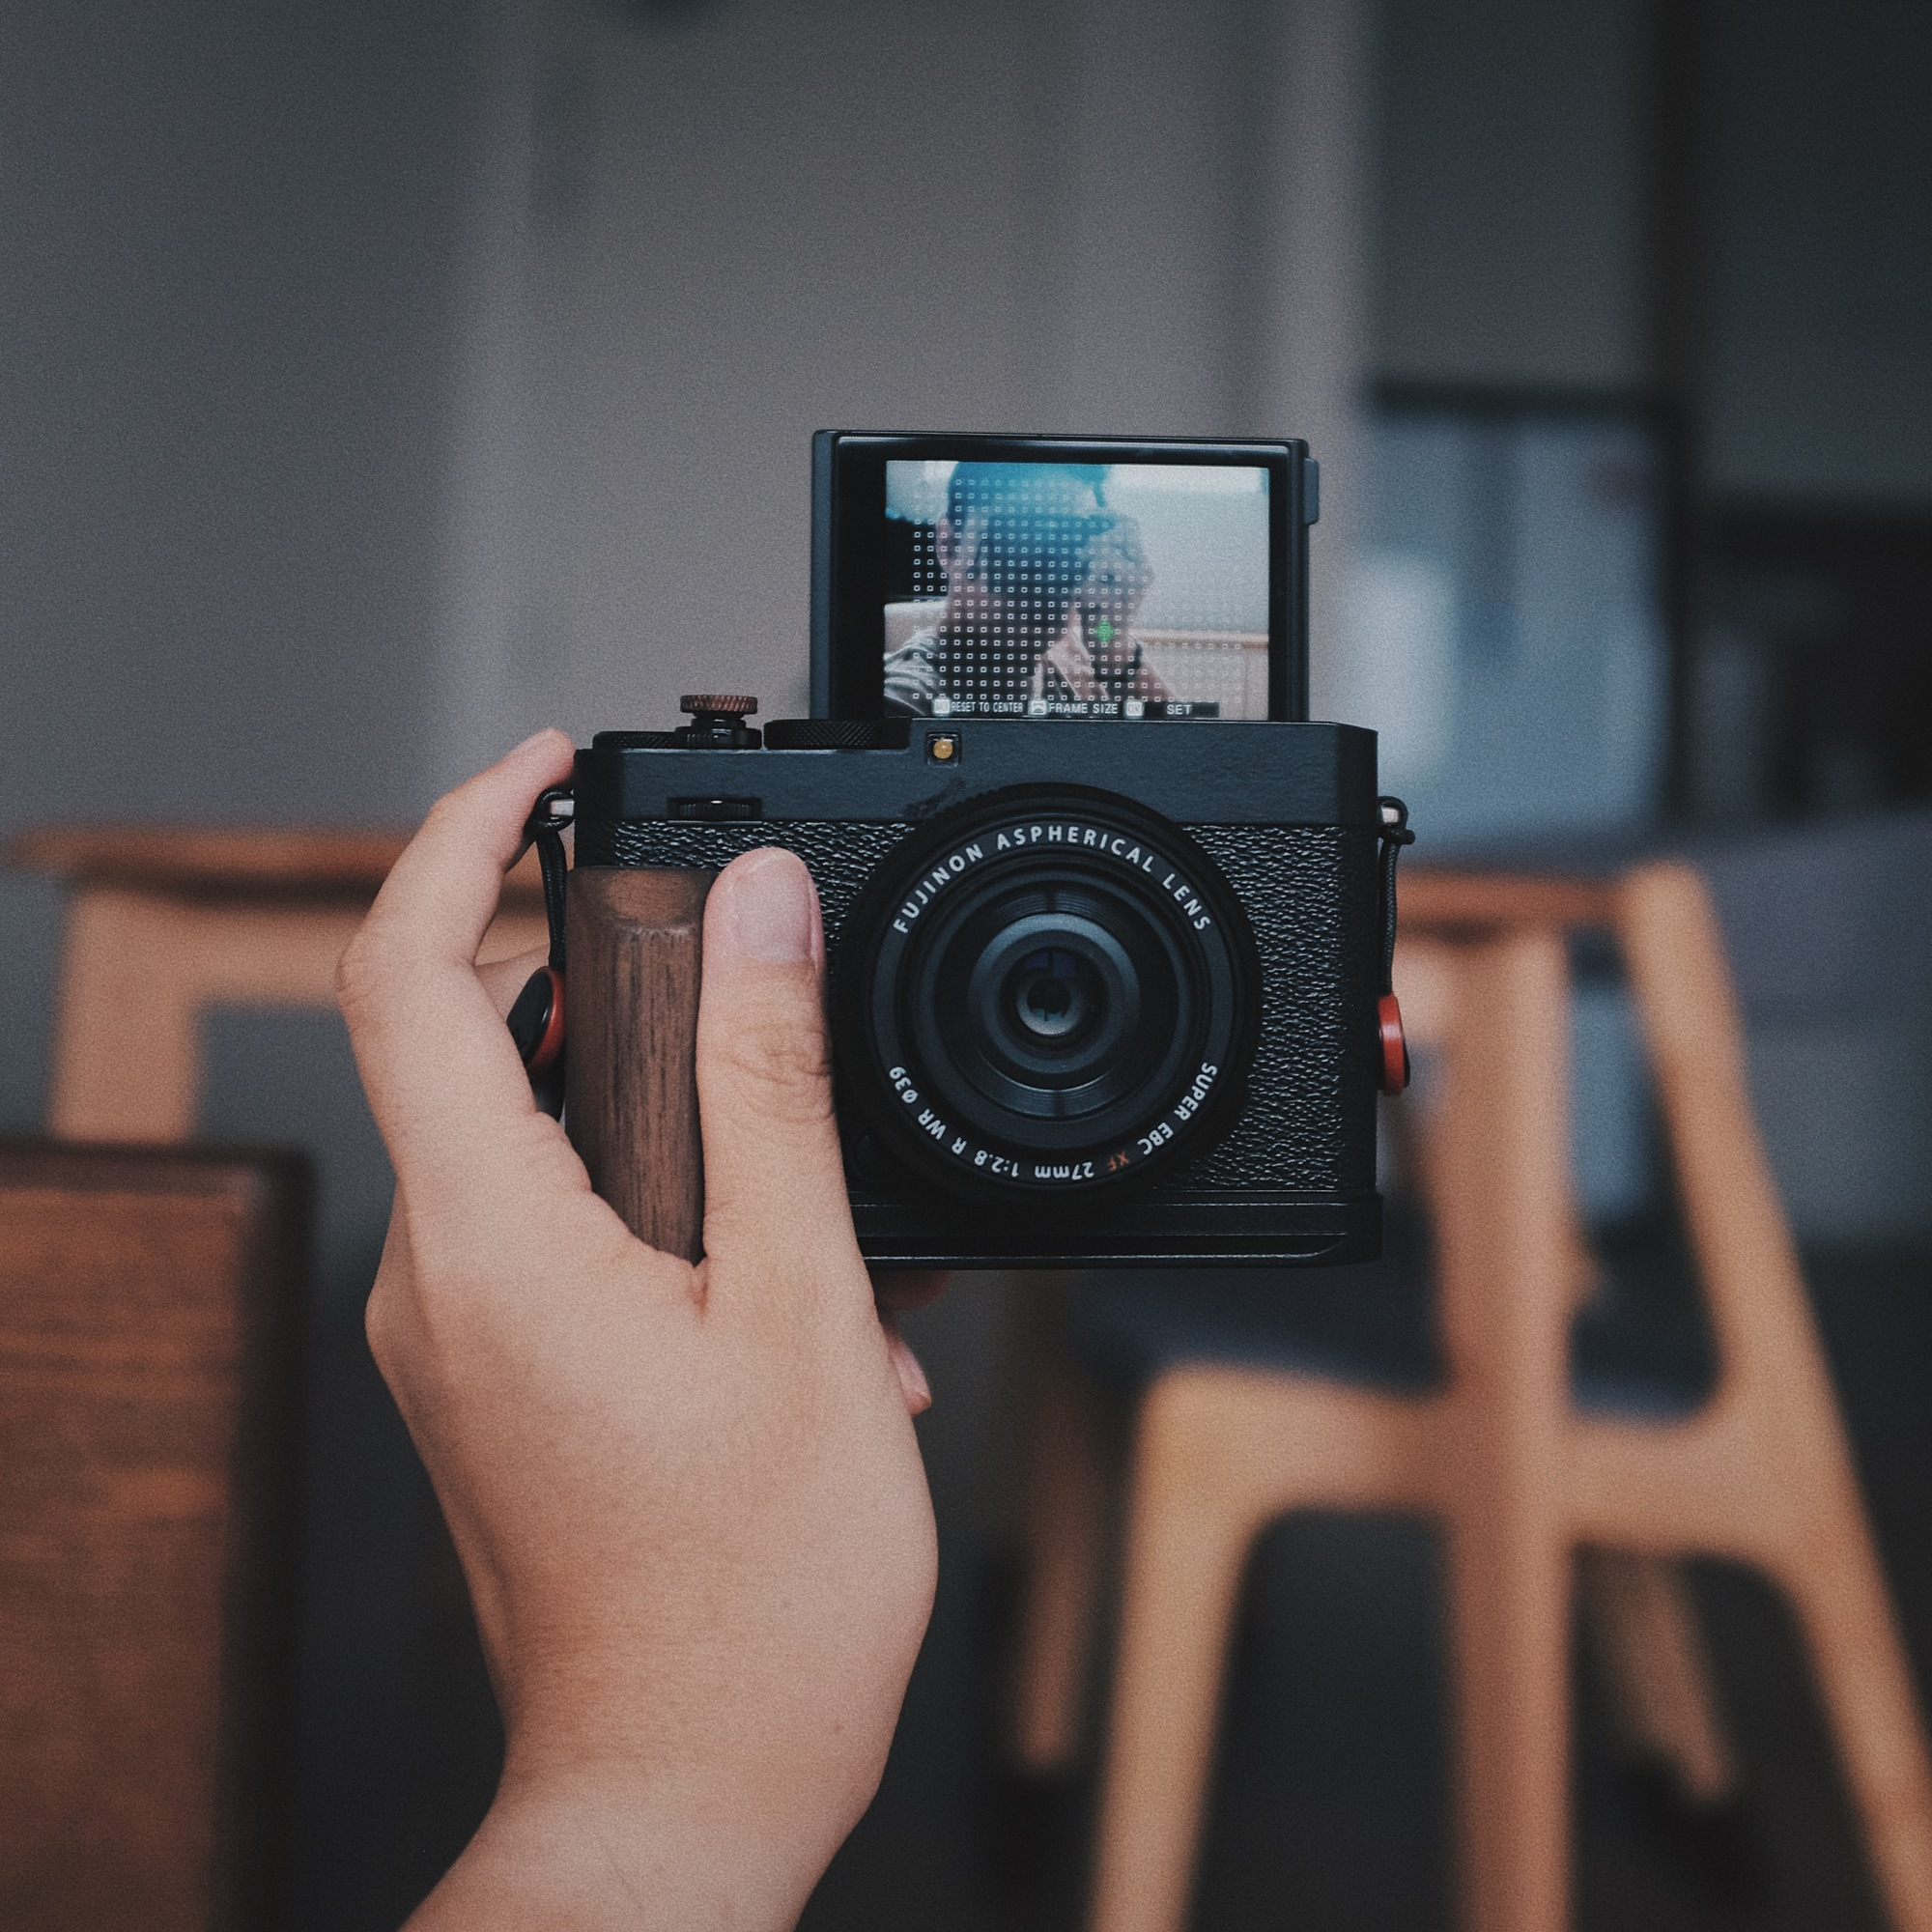
\includegraphics[width=\linewidth]{\envfinaldir/coverpic-prod.jpg}\par
            % \vskip 30pt
            \vfill

            \normalsize\rmfamily\scshape
            \copyright{} The Web Digest Project \hfill\large \envdatestr
        \end{center}
    \end{titlepage}
    % \restoregeometry
}
\newcommand{\simplehref}[1]{%
    \textcolor{blue!80!green}{\href{#1}{#1}}%
}
\renewcommand{\contentsname}{\center\Huge\sffamily\bfseries Contents\par\vskip 20pt}
\newcounter{ipartcounter}
\setcounter{ipartcounter}{0}
\newcommand{\ipart}[1]{
    % \vskip 20pt
    \clearpage
    \stepcounter{ipartcounter}
    \phantomsection
    \addcontentsline{toc}{chapter}{#1}
    % \begin{center}
    %     \Huge
    %     \sffamily\bfseries
    %     #1
    % \end{center}
    % \vskip 20pt plus 7pt
}
\newcounter{ichaptercounter}
\setcounter{ichaptercounter}{0}
\newcommand{\ichapter}[1]{
    % \vskip 20pt
    \clearpage
    \stepcounter{ichaptercounter}
    \phantomsection
    \addcontentsline{toc}{section}{\numberline{\arabic{ichaptercounter}}#1}
    \begin{center}
        \Huge
        \sffamily\bfseries
        #1
    \end{center}
    \vskip 20pt plus 7pt
}
\newcommand{\entrytitlefont}[1]{\subsection*{\raggedright\Large\sffamily\bfseries#1}}
\newcommand{\entryitemGeneric}[2]{
    % argv: title, url
    \parbox{\linewidth}{
        \entrytitlefont{#1}\par\vskip 5pt
        \footnotesize\ttfamily\mdseries
        \simplehref{#2}
    }\vskip 11pt plus 11pt minus 1pt
}
\newcommand{\entryitemGithub}[3]{
    % argv: title, url, desc
    \parbox{\linewidth}{
        \entrytitlefont{#1}\par\vskip 5pt
        \footnotesize\ttfamily\mdseries
        \simplehref{#2}\par\vskip 5pt
        \small\rmfamily\mdseries#3
    }\vskip 11pt plus 11pt minus 1pt
}
\newcommand{\entryitemAp}[3]{
    % argv: title, url, desc
    \parbox{\linewidth}{
        \entrytitlefont{#1}\par\vskip 5pt
        \footnotesize\ttfamily\mdseries
        \simplehref{#2}\par\vskip 5pt
        \small\rmfamily\mdseries#3
    }\vskip 11pt plus 11pt minus 1pt
}
\newcommand{\entryitemHackernews}[3]{
    % argv: title, hnurl, rawurl
    % \parbox{\linewidth}{
    %     \entrytitlefont{#1}\par\vskip 5pt
    %     \footnotesize\ttfamily\mdseries
    %     \simplehref{#3}\par
    %     \textcolor{black!50}{\href{#2}{#2}}
    % }\vskip 11pt plus 11pt minus 1pt
    \begin{minipage}{\linewidth}
            \entrytitlefont{#1}\par\vskip 5pt
            \footnotesize\ttfamily\mdseries
            \simplehref{#3}\par
            \textcolor{black!50}{\href{#2}{#2}}
    \end{minipage}\par\vskip 11pt plus 11pt minus 1pt
}







\begin{document}

\makeheader

\tableofcontents\clearpage




\ipart{Developers}
\ichapter{Hacker News}
\entryitemTwoLinks{FFmpeg devs boast of another 100x leap thanks to handwritten assembly code}{https://news.ycombinator.com/item?id=44629206}{https://www.tomshardware.com/software/the-biggest-speedup-ive-seen-so-far-ffmpeg-devs-boast-of-another-100x-leap-thanks-to-handwritten-assembly-code}

\entryitemTwoLinks{Tough news for our UK users}{https://news.ycombinator.com/item?id=44629134}{https://blog.janitorai.com/posts/3/}

\entryitemTwoLinks{Staying cool without refrigerants: Next-generation Peltier cooling}{https://news.ycombinator.com/item?id=44628930}{https://news.samsung.com/global/interview-staying-cool-without-refrigerants-how-samsung-is-pioneering-next-generation-peltier-cooling}

\entryitemTwoLinks{Payment processors' bar on Japanese adult content endangers democracy (2024)}{https://news.ycombinator.com/item?id=44627828}{https://automaton-media.com/en/news/nier-creator-speaks-out-against-payment-processors-pressuring-japanese-adult-content-platforms/}

\entryitemTwoLinks{Speeding up my ZSH shell}{https://news.ycombinator.com/item?id=44626363}{https://scottspence.com/posts/speeding-up-my-zsh-shell}

\entryitemTwoLinks{XMLUI}{https://news.ycombinator.com/item?id=44625292}{https://blog.jonudell.net/2025/07/18/introducing-xmlui/}

\entryitemTwoLinks{Replit AI deletes entire database during code freeze, then lies about it}{https://news.ycombinator.com/item?id=44625119}{https://twitter.com/jasonlk/status/1946069562723897802}

\entryitemTwoLinks{How Tesla is proving doubters right on why its robotaxi service cannot scale}{https://news.ycombinator.com/item?id=44624952}{https://www.aol.com/elon-gambling-tesla-proving-doubters-090300237.html}

\entryitemTwoLinks{Digital vassals? French Government 'exposes citizens' data to US'}{https://news.ycombinator.com/item?id=44624114}{https://brusselssignal.eu/2025/07/digital-vassals-french-government-exposes-citizens-data-to-us/}

\entryitemTwoLinks{Coding with LLMs in the summer of 2025 – an update}{https://news.ycombinator.com/item?id=44623953}{https://antirez.com/news/154}

\entryitemTwoLinks{A Tour of Microsoft's Mac Lab (2006)}{https://news.ycombinator.com/item?id=44623581}{https://davidweiss.blogspot.com/2006/04/tour-of-microsofts-mac-lab.html}

\entryitemTwoLinks{AI is killing the web – can anything save it?}{https://news.ycombinator.com/item?id=44623361}{https://www.economist.com/business/2025/07/14/ai-is-killing-the-web-can-anything-save-it}

\entryitemTwoLinks{The current hype around autonomous agents, and what actually works in production}{https://news.ycombinator.com/item?id=44623207}{https://utkarshkanwat.com/writing/betting-against-agents/}

\entryitemTwoLinks{A human metaphor for evaluating AI capability}{https://news.ycombinator.com/item?id=44622973}{https://mathstodon.xyz/@tao/114881418225852441}

\entryitemTwoLinks{The bewildering phenomenon of declining quality}{https://news.ycombinator.com/item?id=44622953}{https://english.elpais.com/culture/2025-07-20/the-bewildering-phenomenon-of-declining-quality.html}

\entryitemTwoLinks{LLM architecture comparison}{https://news.ycombinator.com/item?id=44622608}{https://magazine.sebastianraschka.com/p/the-big-llm-architecture-comparison}

\entryitemTwoLinks{Async I/O on Linux in databases}{https://news.ycombinator.com/item?id=44622454}{https://blog.canoozie.net/async-i-o-on-linux-and-durability/}

\entryitemTwoLinks{Show HN: MCP server for Blender that builds 3D scenes via natural language}{https://news.ycombinator.com/item?id=44622374}{https://blender-mcp-psi.vercel.app/}

\entryitemTwoLinks{Borg – Deduplicating archiver with compression and encryption}{https://news.ycombinator.com/item?id=44621487}{https://www.borgbackup.org/}

\entryitemTwoLinks{New York's bill banning One-Person Train Operation}{https://news.ycombinator.com/item?id=44621119}{https://www.etany.org/statements/impeding-progress-costing-riders-opto}


\ipart{Developers~~~~(zh-Hans)}
\ichapter{Solidot}
\entryitemGeneric{\hskip 0pt{}英特尔终止了对 Clear Linux 的支持}{https://www.solidot.org/story?sid=81835}

\entryitemGeneric{\hskip 0pt{}苹果起诉通过进入前员工公寓窃取 iOS 26 机密的 YouTube 主播}{https://www.solidot.org/story?sid=81834}

\entryitemGeneric{\hskip 0pt{}狗看电视的模式}{https://www.solidot.org/story?sid=81833}

\entryitemGeneric{\hskip 0pt{}美国法官允许作家对 Anthropic 盗版数百万电子书提起集体诉讼}{https://www.solidot.org/story?sid=81832}

\entryitemGeneric{\hskip 0pt{}Google 起诉 25 名中国籍 BadBox 2.0 运营者}{https://www.solidot.org/story?sid=81831}

\entryitemGeneric{\hskip 0pt{}俄罗斯新法律将搜索``争议内容''定为犯罪行为}{https://www.solidot.org/story?sid=81830}

\entryitemGeneric{\hskip 0pt{}新闻出版业下线绕过付费墙的服务 12ft.io}{https://www.solidot.org/story?sid=81829}

\entryitemGeneric{\hskip 0pt{}Firefox 141 将支持  WebGPU}{https://www.solidot.org/story?sid=81828}

\entryitemGeneric{\hskip 0pt{}预防工作推动发达国家癌症死亡率下降}{https://www.solidot.org/story?sid=81827}

\entryitemGeneric{\hskip 0pt{}智能手机地震预警不比传统地震监测差}{https://www.solidot.org/story?sid=81826}

\entryitemGeneric{\hskip 0pt{}Netflix 制作《刺客信条》真人剧集}{https://www.solidot.org/story?sid=81825}\ichapter{V2EX}
\entryitemGeneric{\hskip 0pt{}[分享创造] 写了个查看 V2EX 金币趋势的插件}{https://www.v2ex.com/t/1146494}

\entryitemGeneric{\hskip 0pt{}[Apple] 刚发现 Arc 浏览器一个超级厉害又极其简单的功能}{https://www.v2ex.com/t/1146493}

\entryitemGeneric{\hskip 0pt{}[问与答] 大家的独立作品用 ko-fi.com 来设计支付系统吗}{https://www.v2ex.com/t/1146492}

\entryitemGeneric{\hskip 0pt{}[iPhone] iPhone 的浏览器 Safari 的两个问题}{https://www.v2ex.com/t/1146491}

\entryitemGeneric{\hskip 0pt{}[宽带症候群] 在路由器上部署和 一个设备一个客户端 大家更喜欢哪个上网方式?}{https://www.v2ex.com/t/1146490}

\entryitemGeneric{\hskip 0pt{}[问与答] 你们码农是人均家里都有 NAS 吗?大部分人都是为了有个私人网盘?}{https://www.v2ex.com/t/1146489}

\entryitemGeneric{\hskip 0pt{}[程序员] 各位觉得目前最好用、最强大的 agent ai 工具是? Claude Code / Gemini-cli ?}{https://www.v2ex.com/t/1146488}

\entryitemGeneric{\hskip 0pt{}[路由器] 有什么路由器带多播(mDNS), 静态路由设置,同时有 4 lan 口,千兆网}{https://www.v2ex.com/t/1146485}

\entryitemGeneric{\hskip 0pt{}[职场话题] Vibe Coding 时代的职业排序:运营>设计>产品>测试>程序员}{https://www.v2ex.com/t/1146484}

\entryitemGeneric{\hskip 0pt{}[问与答] 求開源的 AI 翻譯和 OCR 工具}{https://www.v2ex.com/t/1146482}

\entryitemGeneric{\hskip 0pt{}[分享发现] 一个好用的 Vim 和 Neovim 配置项目}{https://www.v2ex.com/t/1146481}

\entryitemGeneric{\hskip 0pt{}[前端开发] [求助]webstorm+windsurf 插件 tab 失效的问题}{https://www.v2ex.com/t/1146480}

\entryitemGeneric{\hskip 0pt{}[信息安全] 网站好像中木马了如何处理?}{https://www.v2ex.com/t/1146479}

\entryitemGeneric{\hskip 0pt{}[生活] 暑假弟弟妹妹来家里玩感觉不是很爽}{https://www.v2ex.com/t/1146478}

\entryitemGeneric{\hskip 0pt{}[问与答] 请教,飞牛和威联通共存,配置 UPS 时怎么配置账号密码?}{https://www.v2ex.com/t/1146477}

\entryitemGeneric{\hskip 0pt{}[分享创造] 新手开始学西班牙语,先给自己 DIY 一个学习西班牙字母的网站}{https://www.v2ex.com/t/1146476}

\entryitemGeneric{\hskip 0pt{}[随想] 中医本质上就是大语言模型}{https://www.v2ex.com/t/1146475}

\entryitemGeneric{\hskip 0pt{}[Apple] iPhone 16e 屏幕白色下有杂讯,不够白}{https://www.v2ex.com/t/1146473}

\entryitemGeneric{\hskip 0pt{}[程序员] 小爱音箱是否存在故意"降智"的情况.}{https://www.v2ex.com/t/1146472}

\entryitemGeneric{\hskip 0pt{}[电影] 《长安的荔枝》上映了,咋没人讨论}{https://www.v2ex.com/t/1146470}

\entryitemGeneric{\hskip 0pt{}[分享创造] 画饼: ctrl+F 不好用,我打算写一个浏览器插件,点击后给出一个命令行终端,然后就可以用 grep 等经典工具搜索}{https://www.v2ex.com/t/1146469}

\entryitemGeneric{\hskip 0pt{}[MacBook Pro] 不推荐 14 寸用 m4 max 打游戏,功耗限制导致游戏帧数不如 m3 pro}{https://www.v2ex.com/t/1146468}

\entryitemGeneric{\hskip 0pt{}[阅读] 书籍的英文原版和中文版该如何选择阅读}{https://www.v2ex.com/t/1146466}

\entryitemGeneric{\hskip 0pt{}[硬件] [分享]电蚊拍维修}{https://www.v2ex.com/t/1146465}

\entryitemGeneric{\hskip 0pt{}[问与答] 安卓有哪些好用的浏览器,可以安装扩展}{https://www.v2ex.com/t/1146463}

\entryitemGeneric{\hskip 0pt{}[职场话题] 各位是收到 offer 马上提离职还是等背调完成?}{https://www.v2ex.com/t/1146461}

\entryitemGeneric{\hskip 0pt{}[问与答] iPhone 16e 屏幕不够白}{https://www.v2ex.com/t/1146460}

\entryitemGeneric{\hskip 0pt{}[分享创造] 肝了半天! Gemini CLI 转 API,任意客户端畅享 1000 次/日 Gemini-2.5 请求}{https://www.v2ex.com/t/1146458}

\entryitemGeneric{\hskip 0pt{}[宽带症候群] 家里内网升级到了 2.5g,但是测速总是跑不满}{https://www.v2ex.com/t/1146456}

\entryitemGeneric{\hskip 0pt{}[远程工作] 招聘(远程办公,每个职位 3+ HC): Flutter(app) DevOps  大数据开发工程师 Product Manager Golang 测试工程师 前端工程师(Nodejs / React) Senior HRM}{https://www.v2ex.com/t/1146455}

\entryitemGeneric{\hskip 0pt{}[Cursor] cursor 现在用不了了?}{https://www.v2ex.com/t/1146454}

\entryitemGeneric{\hskip 0pt{}[买买买] 求推荐千元以内办公椅}{https://www.v2ex.com/t/1146453}

\entryitemGeneric{\hskip 0pt{}[问与答] 求推荐随身 WiFi}{https://www.v2ex.com/t/1146450}

\entryitemGeneric{\hskip 0pt{}[I Am A] 程序员转行从事餐饮业近十年,有问必答。}{https://www.v2ex.com/t/1146449}

\entryitemGeneric{\hskip 0pt{}[Apple] 前公司发的 MacBook Pro M2 Max,离职 2 折买入现在属于我个人财产。Apple Care 保 3 年明年过期,不喜欢 macOS 几乎没怎么用,电池健康 94\%,可以续保到过时产品然后申请免费换新吗?}{https://www.v2ex.com/t/1146447}

\entryitemGeneric{\hskip 0pt{}[分享发现] 兄弟们,阿里小号要关了,赶紧找下家吧}{https://www.v2ex.com/t/1146446}

\entryitemGeneric{\hskip 0pt{}[硬件] 25 年 4K 显示器选择}{https://www.v2ex.com/t/1146445}

\entryitemGeneric{\hskip 0pt{}[问与答] 求助论坛大佬: marktext 编辑 Markdown 时总是会把多个空行合并为一个空行如何解决?}{https://www.v2ex.com/t/1146443}

\entryitemGeneric{\hskip 0pt{}[Apple] 主打听劝,换了个路由器}{https://www.v2ex.com/t/1146442}

\entryitemGeneric{\hskip 0pt{}[加密货币] hyperliquid 会支持合约网格交易么?}{https://www.v2ex.com/t/1146440}

\entryitemGeneric{\hskip 0pt{}[iPad] iPad Pro 2018 被列入过时产品}{https://www.v2ex.com/t/1146439}

\entryitemGeneric{\hskip 0pt{}[Minecraft] 极限生存 1.21.4 互通服( Java )}{https://www.v2ex.com/t/1146438}

\entryitemGeneric{\hskip 0pt{}[Telegram] 我开发了一个使用 Github 一站式记录和管理笔记的 Telegram Bot,欢迎大家使用}{https://www.v2ex.com/t/1146437}

\entryitemGeneric{\hskip 0pt{}[API] 网页 URL 转 Markdown API 接口}{https://www.v2ex.com/t/1146436}

\entryitemGeneric{\hskip 0pt{}[生活] 为什么越是穷苦的人,越是有同理心……}{https://www.v2ex.com/t/1146435}

\entryitemGeneric{\hskip 0pt{}[Visual Studio Code] cursor 怎么同步配置方便}{https://www.v2ex.com/t/1146434}

\entryitemGeneric{\hskip 0pt{}[Docker] WSL 中无法访问 registry-1.docker.io/v2/,没法用 docker 拉取 image,试了很多方法都不行,累了}{https://www.v2ex.com/t/1146433}

\entryitemGeneric{\hskip 0pt{}[问与答] EDA 也接入 AI agent 了,这下是不是搞硬件的也会被 AI 替代部分了}{https://www.v2ex.com/t/1146432}

\entryitemGeneric{\hskip 0pt{}[酷工作] [上海]TEMU 招 web 前端工程师}{https://www.v2ex.com/t/1146430}

\entryitemGeneric{\hskip 0pt{}[宽带症候群] 广州城中村宽带太气人了}{https://www.v2ex.com/t/1146429}


\ipart{Generic News}
\ichapter{Reuters}
\entryitemWithDescription{\hskip 0pt{}Trump administration pushes states for election data, Washington Post reports}{https://www.reuters.com/world/us/trump-administration-pushes-states-election-data-washington-post-reports-2025-07-16/}{The Trump administration and its allies are trying to obtain voter data from states and inspect voting equipment, the Washington Post reported on Wednesday, in moves it said had caused concern among state and local election...}

\entryitemWithDescription{\hskip 0pt{}Returned deportee Abrego due in Tennessee court; future of smuggling case uncertain}{https://www.reuters.com/legal/government/returned-deportee-abrego-due-tennessee-court-future-smuggling-case-uncertain-2025-07-16/}{Federal prosecutors are seeking to convince District Judge Waverly Crenshaw to reverse a magistrate judge's ruling allowing Kilmar Abrego to be released on bail to await a...}

\entryitemWithDescription{\hskip 0pt{}Exclusive: US considered charging Minnesota judges, lawyers in immigration crackdown, sources say}{https://www.reuters.com/legal/government/us-considered-charging-minnesota-judges-lawyers-immigration-crackdown-sources-2025-07-16/}{The judges and defense lawyers discussed requesting virtual court hearings to protect defendants from being arrested by federal immigration...}

\entryitemWithDescription{\hskip 0pt{}Trump, White House race to stem Epstein conspiracy fallout}{https://www.reuters.com/business/media-telecom/trump-white-house-race-stem-epstein-conspiracy-fallout-2025-07-16/}{The persisting furor over files related to accused sex trafficker Jeffrey Epstein has forced President Donald Trump into an unfamiliar role: trying to shut a conspiracy theory...}

\entryitemWithDescription{\hskip 0pt{}US says it has sent third-country deportees to Southern Africa's Eswatini}{https://www.reuters.com/world/us/us-says-it-has-sent-third-country-deportees-southern-africas-eswatini-2025-07-16/}{The U.S. Homeland Security Department said on Tuesday a deportation flight carrying immigrants from different countries had landed in Eswatini, in a move that follows the U.S. Supreme Court lifting limits on deporting migrants to third...}

\entryitemWithDescription{\hskip 0pt{}Trump: Bessent an option to replace Fed chair, 'but I like the job he's doing'}{https://www.reuters.com/world/us/trump-bessent-an-option-replace-fed-chair-but-i-like-job-hes-doing-2025-07-15/}{President Donald Trump said on Tuesday that Treasury Secretary Scott Bessent could be a candidate to replace Federal Reserve Chairman Jerome Powell, but suggested that might not...}

\entryitemWithDescription{\hskip 0pt{}US Republicans grill university leaders in latest House antisemitism hearing}{https://www.reuters.com/legal/government/us-republicans-grill-university-leaders-latest-house-antisemitism-hearing-2025-07-15/}{The leaders of three U.S. universities testified before a House of Representatives panel on Tuesday about what they have done to combat antisemitism on campus, saying they were committed to stamping out hatred while protecting academic...}

\entryitemWithDescription{\hskip 0pt{}Trump administration sues to oust Corporation for Public Broadcasting board members}{https://www.reuters.com/business/media-telecom/trump-administration-sues-oust-corporation-public-broadcasting-board-members-2025-07-15/}{President Donald Trump\textquotesingle s administration filed a lawsuit on Tuesday against three board members of the Corporation for Public Broadcasting who have not left their posts despite Trump\textquotesingle s attempt to fire...}

\entryitemWithDescription{\hskip 0pt{}Former US Army soldier pleads guilty in phone company hacking, extortion case}{https://www.reuters.com/legal/government/former-us-army-soldier-pleads-guilty-phone-company-hacking-extortion-case-2025-07-15/}{A former U.S. Army soldier pleaded guilty on Tuesday to hacking telecommunications companies\textquotesingle{} databases, stealing records, and demanding ransoms for the stolen data, the U.S. Department of Justice...}

\entryitemWithDescription{\hskip 0pt{}Trump backs Texas plan to redraw voting maps to benefit House Republicans}{https://www.reuters.com/world/us/trump-backs-texas-plan-redraw-voting-maps-benefit-house-republicans-2025-07-15/}{President Donald Trump on Tuesday said he believed Republicans could pick up five seats in the U.S. House of Representatives by redrawing districts in Texas, which could boost his party\textquotesingle s odds of defending its thin...}

\entryitemWithDescription{\hskip 0pt{}US military to remove 2,000 National Guard troops from Los Angeles}{https://www.reuters.com/world/us/us-military-remove-2000-national-guard-troops-los-angeles-2025-07-15/}{U.S. Defense Secretary Pete Hegseth has ordered the removal of half of the 4,000 National Guard troops who had been sent to Los Angeles to protect federal property and personnel during a spate of protests last month, the Pentagon said on...}

\entryitemWithDescription{\hskip 0pt{}White House National Security Council hit by more departures, sources say}{https://www.reuters.com/world/us/white-house-national-security-council-hit-by-more-departures-sources-say-2025-07-15/}{Two senior officials at the White House National Security Council have left their roles in recent days, according to two sources familiar with the moves, the latest departures for a body that has been cut sharply in recent...}

\entryitemWithDescription{\hskip 0pt{}US opens probe into University of Michigan's foreign funding}{https://www.reuters.com/world/us/us-education-department-opens-foreign-funding-probe-into-university-michigan-2025-07-15/}{The U.S. Education Department said on Tuesday it opened a foreign funding investigation into the University of Michigan while alleging it found "inaccurate and incomplete disclosures" in a review of the university\textquotesingle s...}






\clearpage
\leavevmode\vfill
\footnotesize

Copyright \copyright{} 2023-2025 Neruthes and other contributors.

This document is published with CC BY-NC-ND 4.0 license.

The entries listed in this newsletter may be copyrighted by their respective creators.

This newsletter is generated by the Web Digest project.

The newsletters are also delivered via Telegram channel \CJKunderline{\href{https://t.me/webdigestchannel}{https://t.me/webdigestchannel}}.\\
RSS feed is available at \CJKunderline{\href{https://webdigest.pages.dev/rss.xml}{https://webdigest.pages.dev/rss.xml}}.

This newsletter is available in PDF at
\CJKunderline{\href{https://webdigest.pages.dev/}{https://webdigest.pages.dev/}}.

The source code being used to generate this newsletter is available at\\
\CJKunderline{\href{https://github.com/neruthes/webdigest}{https://github.com/neruthes/webdigest}}.

This newsletter is also available in
\CJKunderline{\href{http://webdigest.pages.dev/readhtml/\envyear/WebDigest-20250721.html}{HTML}} and
\CJKunderline{\href{https://github.com/neruthes/webdigest/blob/master/markdown/\envyear/WebDigest-20250721.md}{Markdown}}.


\coverpic{https://unsplash.com/photos/modern-building-with-car-parked-in-front-jKNSliPAV0g}{Luke Miller}


\end{document}
